\newcommand{\rendering}[1]{
  \includegraphics[height=\renderingheight]{assets/\clogdirname/pipeline/image_#1.png}
}
\newcommand{\uvmap}[1]{
  \includegraphics[height=\uvheight]{assets/\clogdirname/pipeline/interpolation_#1.png}
}
\newcommand{\modulateduvmap}[1]{
  \includegraphics[height=\renderingheight]{assets/\clogdirname/pipeline/modulated_pred_#1.png}
}
\newcommand{\unmodulateduvmap}[1]{
  \includegraphics[height=\renderingheight]{assets/\clogdirname/pipeline/unmodulated_pred_#1.png}
}
\newcommand{\clogpipelinefig}{
  \def\inputheight{128bp}
  \def\renderingheight{64bp}
  \def\preplasheight{78bp}
  \def\uvheight{52bp}
  \centering
  \font\nullfont=cmr10
  \tikzsetnextfilename{clogpipeline}
  \tikzset{external/export next=false}
  \resizebox{\linewidth}{!}{
    \begin{tikzpicture}[
        >=stealth',
        overlay/.style={
            anchor=south west,
            draw=black,
            rectangle,
            line width=0pt,
            outer sep=0,
            inner sep=0,
          },
      ]
      \node (data) {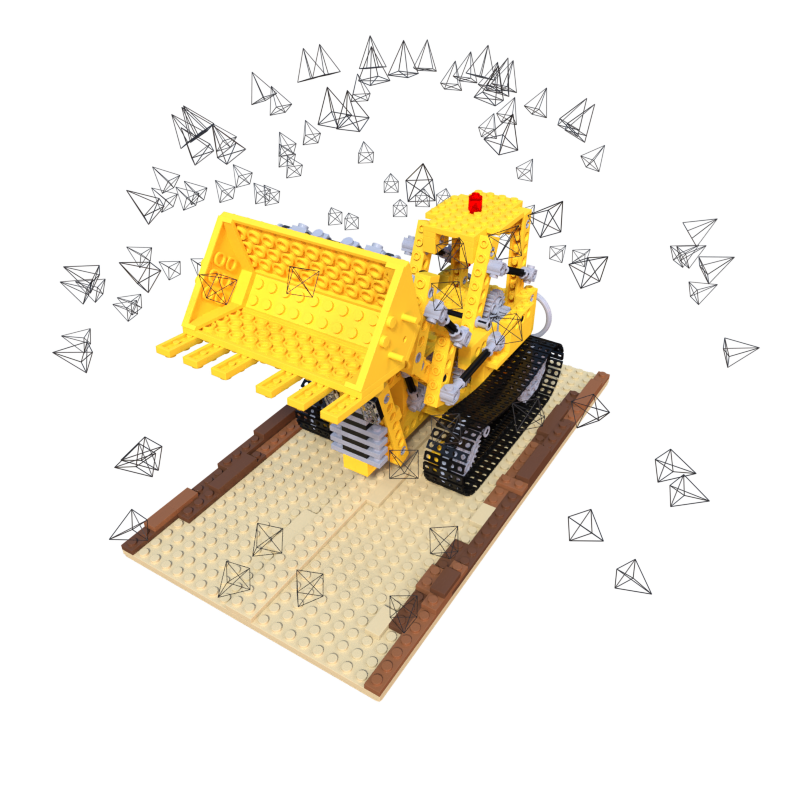
\includegraphics[height=\inputheight]{assets/\clogdirname/pipeline/vis.png}};

      \matrix[
        matrix of nodes,
        right=1em of data,
        column sep=0pt,
        row sep=1.4em,
        ampersand replacement=\&,
        inner sep=0,
        outer sep=0
      ] (pictures) {
        \rendering{0.00} \&
        \rendering{0.25} \&
        \rendering{0.50} \&
        \rendering{0.75} \&
        \rendering{1.00} \\
        \uvmap{0.00} \&
        \uvmap{0.25} \&
        \uvmap{0.50} \&
        \uvmap{0.75} \&
        \uvmap{1.00}     \\
      };
      \node[above right=0em and 0.2em of pictures-2-1.north, scale=0.4] (firstnet) {\rotatebox{90}{\usebox\neuralnet}};
      \node[above=-0.4em of firstnet.north] {\smaller \cref{eq:clog-decoders}};
      \node[above right=0em and 0.2em of pictures-2-2.north, scale=0.4]{\rotatebox{90}{\usebox\neuralnet}};
      \node[above right=0em and 0.2em of pictures-2-3.north, scale=0.4]{\rotatebox{90}{\usebox\neuralnet}};
      \node[above right=0em and 0.2em of pictures-2-4.north, scale=0.4]{\rotatebox{90}{\usebox\neuralnet}};
      \node[above right=0em and 0.2em of pictures-2-5.north, scale=0.4]{\rotatebox{90}{\usebox\neuralnet}};

      \node[right=-1em of data.west, align=center, anchor=base] (stageone) {\rotatebox{90}{Stage I}};
      \node[right=-1.5em of pictures-2-1.west, align=center]{\rotatebox{90}{\smaller Grid of Latents~$\cloglatents$}};
      \node[above=0em of data.north, align=center] {Calibrated cameras};

      \draw[-stealth,  thick, dashed,  ->] ([yshift=4pt]pictures-1-1.north west) -- node [above, midway] {\smaller Training progression and upsampling~(\cref{eq:clog-upsampling})} ([yshift=4pt]pictures-1-5.north east);

      \node[right=1em of pictures.east] (preplas) {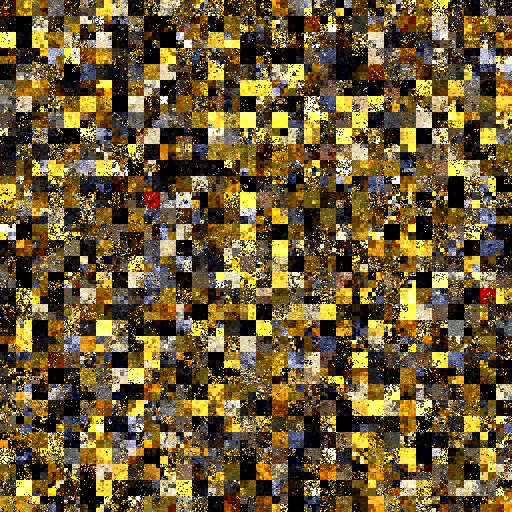
\includegraphics[height=\inputheight]{assets/\clogdirname/plas/unsorted_colors.png}};
      \node[below=3em of preplas.south] (postplas) {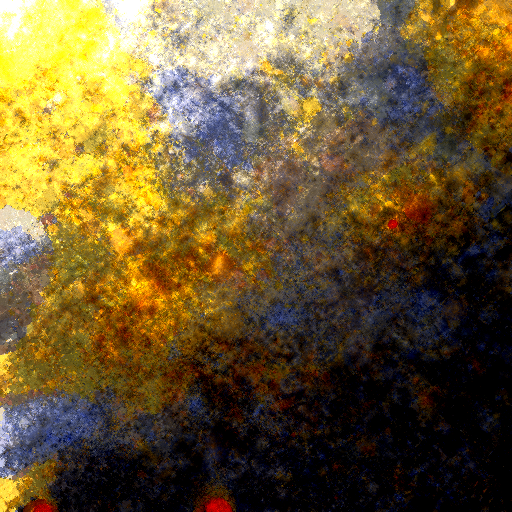
\includegraphics[height=\inputheight]{assets/\clogdirname/plas/sorted_colors.png}};k
      \node[above=0em of preplas.north, align=center] {Trained Grid};

      \draw[-stealth, shorten >= 1pt, shorten <= 1pt,  thick,  ->] (preplas.south) -- node [right, midway] {\smaller PLAS~\cite{morgenstern2024compact}}(postplas.north);

      \node[above left=0.25em and 3.5em of postplas, anchor=north east, scale=1.15] (modulator) {\rotatebox{180}{\usebox\neuralnet}};

      \matrix[
        matrix of nodes,
        left=12em of postplas.west,
        column sep=0pt,
        row sep=0em,
        ampersand replacement=\&,
        inner sep=0,
        outer sep=0
      ] (secondstage) {
        \modulateduvmap{0.00} \&
        \modulateduvmap{0.25} \&
        \modulateduvmap{0.50} \&
        \modulateduvmap{0.75} \&
        \modulateduvmap{1.00}   \\
        \unmodulateduvmap{0.00} \&
        \unmodulateduvmap{0.25} \&
        \unmodulateduvmap{0.50} \&
        \unmodulateduvmap{0.75} \&
        \unmodulateduvmap{1.00} \\
      };
      \draw[-stealth, decoration={snake, pre length=0.01mm, segment length=2mm, amplitude=0.3mm, post length=1.5mm}, decorate, thick] ([yshift=-32bp]postplas.west) -- node [above, midway] {No modulation} (secondstage-2-5);

      \draw[-stealth, decoration={snake, pre length=0.01mm, segment length=2mm, amplitude=0.3mm, post length=1.5mm}, decorate, thick] ([yshift=32bp]postplas.west) -- node [above, midway] {\cref{eq:clog-modulator}} (modulator.east);
      \draw[-stealth, decoration={snake, pre length=0.01mm, segment length=2mm, amplitude=0.3mm, post length=1.5mm}, decorate, thick] (modulator.west) -- node [above, midway] {\cref{eq:clog-modulating}} (secondstage-1-5);

      \node[above=-0.5em of modulator] {Our modulator $\modulator$};

      \node[below=18em of stageone.south, align=center, anchor=base] {\rotatebox{90}{Stage II}};

      \draw[-stealth,  thick, dashed,  ->] ([yshift=0pt]secondstage-1-5.north east) -- node [above, midway] {\smaller Decreasing LoD~$\lod\in[0, 1]$} ([yshift=0pt]secondstage-1-1.north west);

      \node[right=-1.5em of secondstage-1-1.west, align=center] {\small\rotatebox{90}{\textbf{Ours}}};
      \node[right=-1.5em of secondstage-2-1.west, align=center] {\small\rotatebox{90}{For comparison}};

    \end{tikzpicture}
  }
}
\begin{figure}
  \centering
  \clogpipelinefig
  \caption{
    \textbf{Pipeline --}
    We represent the scene with a 2D UV map containing features that an MLP
    interprets 3D Gaussians.
    We first train the UV map at the highest resolution and sort it to ensure
    spatial coherence of similar features, enabling effective subsampling.
    For any desired level of detail (LoD), we obtain the corresponding UV map
    by downsampling and processing it through a modulator that adapts the
    features to map correctly to 3D Gaussians at reduced density.
    This approach enables support for \emph{arbitrary} levels of detail.
  }
  \label{fig:clog-pipeline}
\end{figure}